%%%%%%%%%%%%%%%%%%%%%%%%%%%%%%%%%%%%%%%
% Ch3 : Introduction to heat transfer %
%%%%%%%%%%%%%%%%%%%%%%%%%%%%%%%%%%%%%%%

\chapter{Heat transfer}
\section{Introduction}
	We retrieve heat transfer in many phenomena like the combustion of coal that we use for the barbecue, the steel production or in power plants. But thermodynamics don't tell us how fast combustion will take place, chemistry tells us it will go too fast and each reaction needs its own reaction rate. \\
	Heat transfer is important in the duration of many processes. It's important to design and understand that principle for engineers. 
	
	\subsection{Definitions}
	\subsubsection{Energy}
		\begin{center}
		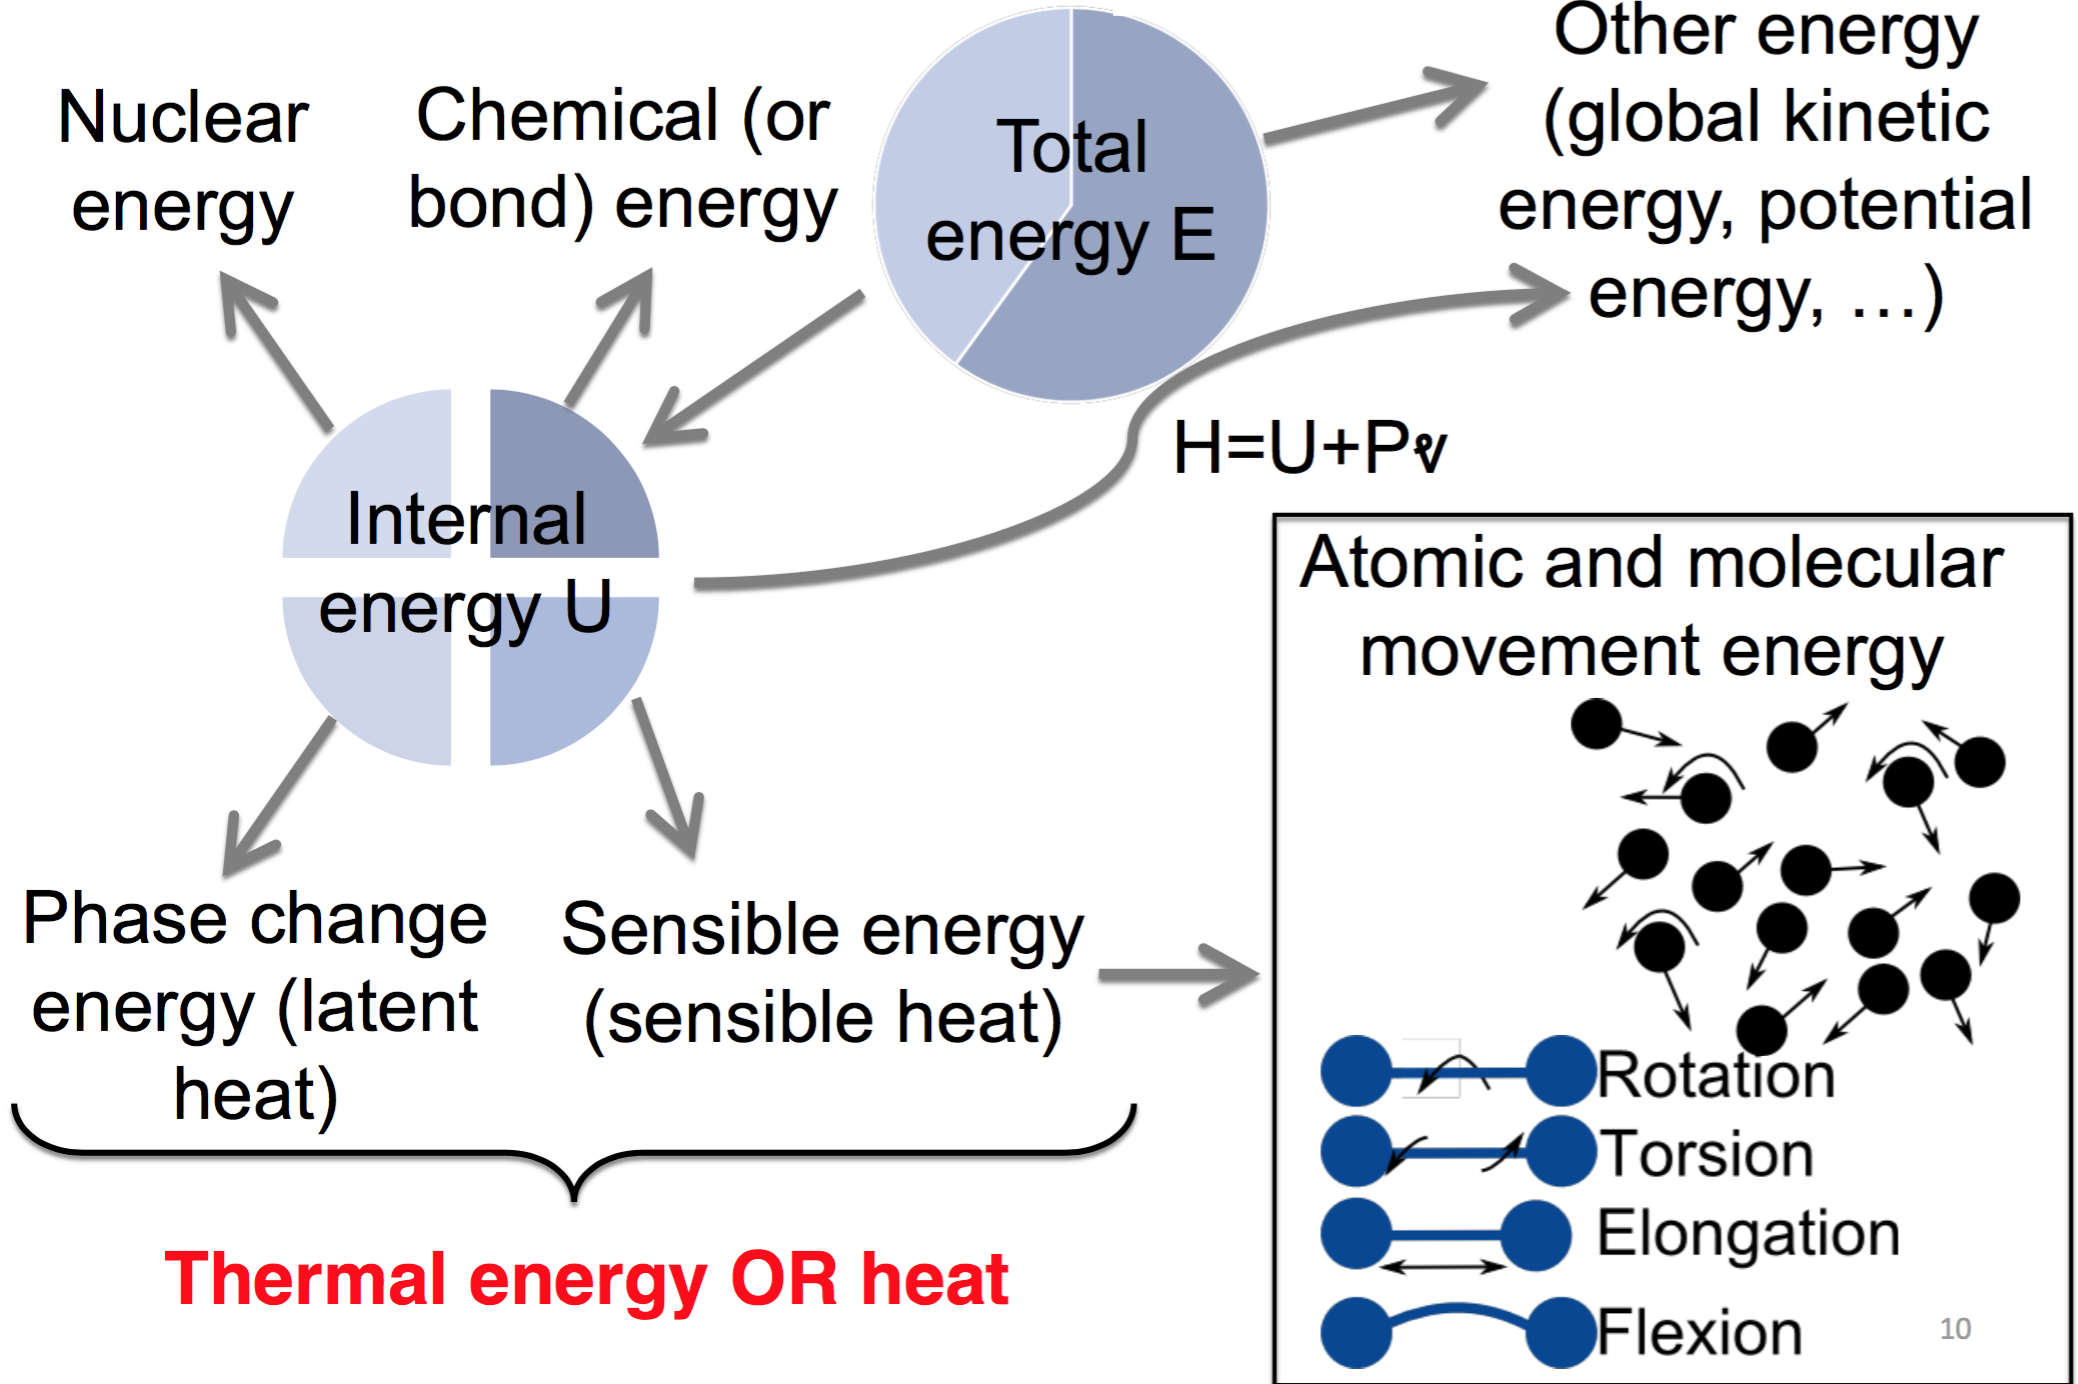
\includegraphics[scale=0.25]{ch3/1}
		\end{center}
		In a system you have the total energy and is divided in two : internal energy and the rest. The first is the energy you find in the system if you attach yourself to the system. Thermal energy or heat includes the \textbf{latent heat} that is the phase change energy and the \textbf{sensible heat} that is associated to the atomic move inside the material. 
		
	\subsubsection{Temperature}
		It's an interesting principle because it's not simple to define it. You can have thermodynamic definition of temperature : linked to the entropy (system is changing) and microscopic theory linked to the move of particles. \\
		The important for us is that temperature is an intensive quantity correlated to the internal energy of the system. It's a universal feature of matters so it's independent of the material. \\
		Temperature is linked to the system energy by the specific heat 
		\begin{equation}
			dU = mc_v dT \qquad and \qquad dH = mc_p dT
		\end{equation}

		Should remember that gas of low pressure and low velocity can be considered as incompressible. In that case 
		\begin{equation}
			c_v = c_p = c
		\end{equation}		 
		
	\subsubsection{Heat flux}
		With 2 bodies at different temperatures in contact, a quantity $Q(J)$ of heat is transferred through a surface of area $A$. Heat transfer rate and heat transfer flux density are defined as 
		\begin{equation}
			\dot{Q} = \frac{dQ}{dt} \qquad \Rightarrow \qquad \dot{q} = \frac{\dot{Q}}{A}
		\end{equation}
		
\subsection{Heat balance}
		The idea is to see what heat induct. Heat is just a part of energy in the system, only the total energy is conserved. What we will do is make balances on a control volume but we will divide the energy in two parts (heat and the rest). We will take into account the heat flux entrance and exit on a control volume surface, the generation or the consumption and the accumulation :
		\begin{equation}
			\mbox{accumulation} + \mbox{out fluxes} + \mbox{sinks} = \mbox{sources} + \mbox{in fluxes}
			\label{eq:3.4}
		\end{equation}
		Sources and sinks can be due to the transformation of heat energy into a non thermal energy (sinks) or vice versa (source). \\
		We can divide the situation in 2. The one where we accumulate and the other where we don't. The first case corresponds to stationary systems. The difference between \textbf{stationary }and \textbf{equilibrium} is that the second is a particular stationary state where we have no flux whereas they are present in a stationary flux. 

 \subsection{Heat transfer mechanisms}
 	\subsubsection{Conduction}
 		Universal heat transfer by contact. It appears in matter when molecules enter in contact with each others and transfer heat. The entropic transport of heat is quite slow. Universal because it can happen everywhere we have matter and is the main heat transfer. Solid materials are characterized as good heat conductor or not, so it's a material property.
 
 	\subsubsection{Convection}
 		\begin{wrapfigure}[6]{r}{1cm}
 		\vspace{-5mm}
 		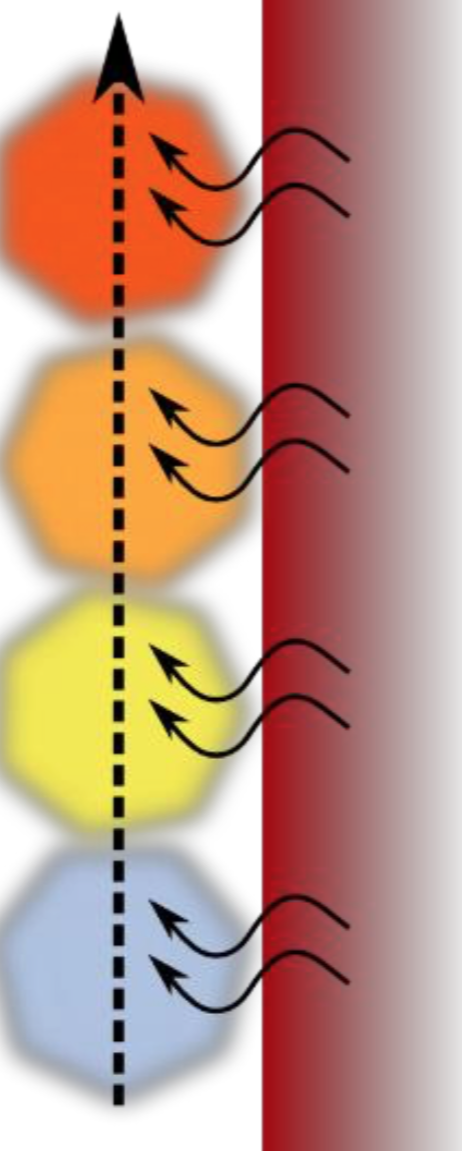
\includegraphics[scale=0.15]{ch3/2}
 		\end{wrapfigure}
		Convection is linked to the movement of the particles but they carry they own heat. During this movement conduction occurs : convection = conduction + advection (illustrated on the picture). It's the major transfer in presence of flows. Convection is complicated, it depends on how moves the fluid, its direction, ... (dependent). \\
		We have to do the difference between forced and natural convection. For forced convection, the flow exists even if there is no heat transfer whereas for natural convection the flow is due to the heat transfer. 
		
		\subsubsection{Radiation}
		It's the electromagnetic waves heat transfer between surfaces far from each other. No need to have matter, it's important to have a large temperature difference. It's more complex mathematically but we often neglect it.
		
	\section{Conduction}
		\subsection{Microscopic approach}
			\begin{wrapfigure}[8]{l}{3cm}
 			\vspace{-5mm}
 			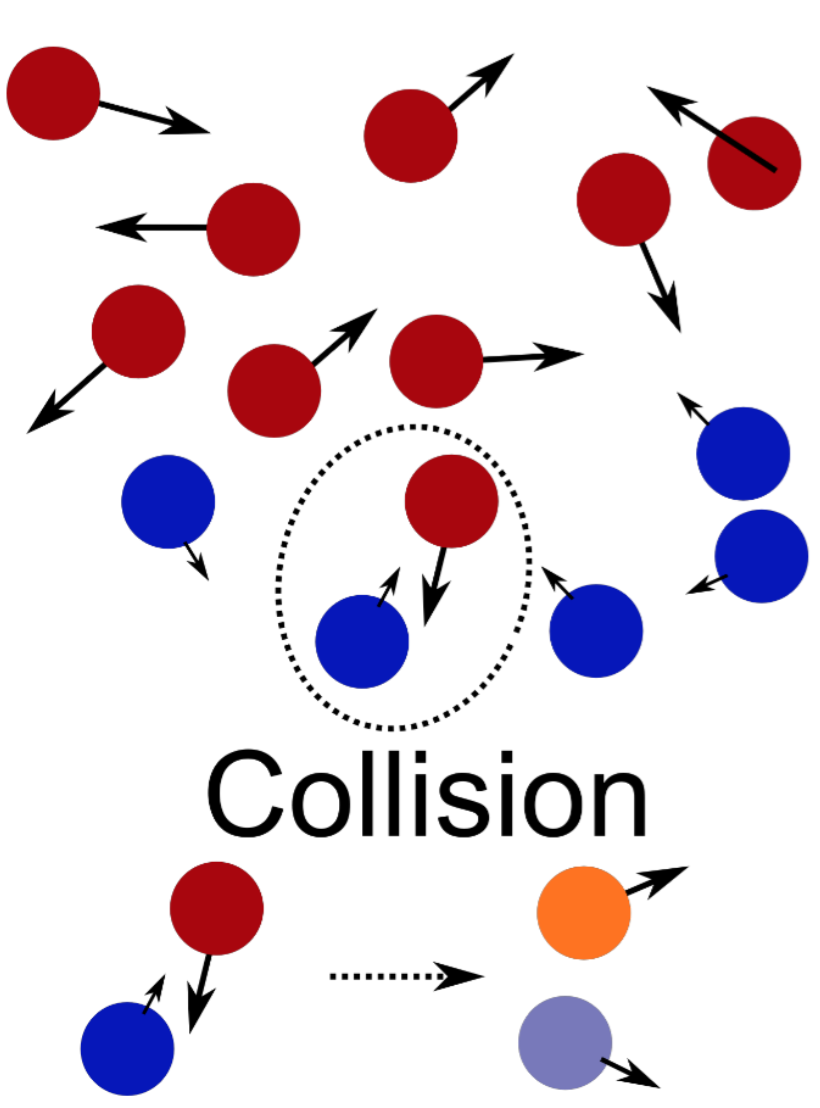
\includegraphics[scale=0.2]{ch3/3}
 			\end{wrapfigure}
 			Temperature is an indicator of the particles movement. Hot bodies are composed of particles faster than cold bodies and when they are placed in contact, collisions occur, leading the hotter particle to transfer kinetic energy and so heat to the colder one. \\
 			The higher the temperature gradient is, the faster the transfer will be. This transfer process continues until the equalization of temperature and the quantity transferred depends on the temperature, the chemical compositions and the densities.
 			
 		\subsection{Phenomenological approach - the first Fourier law}
 			\begin{wrapfigure}[8]{r}{3cm}
 			\vspace{-5mm}
 			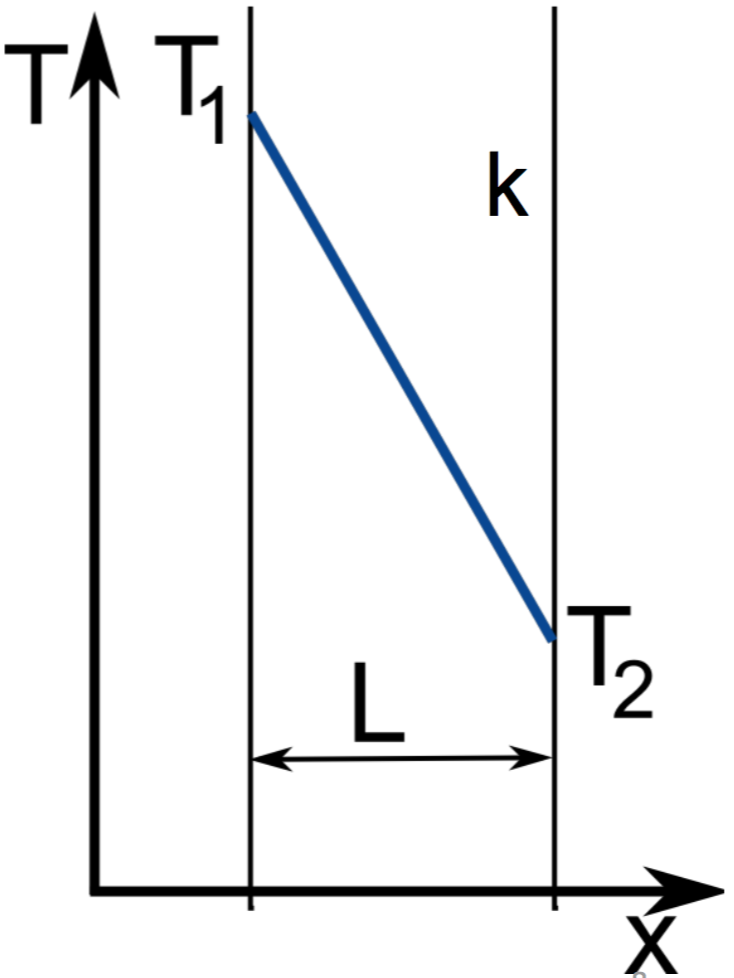
\includegraphics[scale=0.2]{ch3/4}
 			\end{wrapfigure}
 			Let's take an infinite wall of thickness $L$. We fix two temperature and we look at the temperature profile of the system. The amount of heat transfer will be proportional to the thermal conductibility $k \, [W/m.K]$  and the heat flux density is 
 			\begin{equation}
 				\dot{q} = k \frac{T_1-T_2}{L}
 			\end{equation}
 			We can consider the thickness equal to $L = -dx$ giving
 			\begin{equation}
 				\dot{q} = -k\frac{dT}{dx}
 			\end{equation}
 			
 		\subsection{Thermal conductibility and diffusivity}
			\subsubsection{Thermal diffusivity} 	
	 			$k$ is mainly dependent of the materials properties but includes the thermal capacity. So we can express a value called \textbf{thermal diffusivity} defined as (unity : $m^2/s$)
 				\begin{equation}
 					\alpha = \frac{k}{\rho C_p}
 					\label{eq:3.7}
 				\end{equation}
 			
	 		\subsubsection{Thermal conductivity of materials}
	 			\begin{itemize}
	 				\item[•] \textbf{Gas :} particles are far from each other, so there are few collision and so few transfer by conduction. 
	 				\item[•] \textbf{Liquid :} many random shocks giving better conduction skills. 
	 				\item[•] \textbf{Solid :} the rigidity makes from them bad conductors but the crystals can transfer heat fast. They can so be good conductors or insulators\footnote{Isolant}. \\
	 			\end{itemize}
	 			
	 			$k$ has some dependence with temperature that is neglect for small changes. \textbf{We have to beware of phase changes!}
	 			
	 	\section{1D stationary conductive heat balance}
	 		\begin{wrapfigure}[8]{l}{2.2cm}
 			\vspace{-5mm}
 			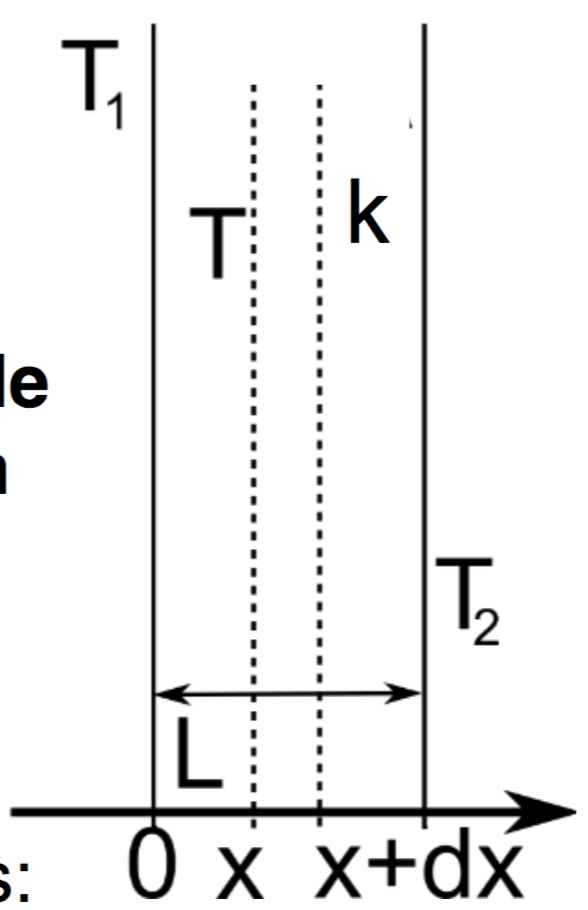
\includegraphics[scale=0.2]{ch3/5}
 			\end{wrapfigure}
 			Let's apply a heat balance on the walls of thickness $dx$ using equation \autoref{eq:3.4}. There is no source and no accumulation term. 
 			\begin{equation}
 				\mbox{Flux In = Flux out} \qquad \Leftrightarrow \qquad A\dot{q}_x = A\dot{q}_{x+dx}
 				\label{eq:3.8}
 			\end{equation}
 			With a first order Taylor expansion we have the expression of $\dot{q}_{x+dx}$ and replaced in \autoref{eq:3.8}
 			\begin{equation}
 				\dot{q}_{x+dx} = \dot{q}_x + \frac{d\dot{q}_x}{dx}dx \qquad \Rightarrow \qquad \frac{d\dot{q}_x}{dx} = 0
 			\end{equation}
 			We apply the Fourier Law ($k =cst$)
 			\begin{equation}
 				\frac{d\dot{q}_x}{dx} = \frac{d}{dx}\left(- k\frac{dT}{dx} \right) = \frac{d^2T}{dx^2} = 0 \qquad \Rightarrow \qquad T = C_1 x + C_2
 			\end{equation}
 			\subsection{Heat resistance}
	 			The boundary conditions $T =T_1$ for $x = 0$ and $T=T_2$ for $x=L$ gives the constants, so
 				\begin{equation}
 					T = \frac{T_2-T_1}{L}x + T_1
 				\end{equation}
 				If we reapply the Fourier Law (deriving the equation above) 
 				\begin{equation}
	 				\dot{q} = k\frac{T_1 -T_2}{L}
 				\end{equation}
 				We define now the \textbf{thermal resistance} of the wall $R = \frac{L}{kA}$ and obtain the heat transfer rate 
 				\begin{equation}
 					\dot{Q} = \frac{T_1 - T_2}{R}
 				\end{equation}
 				
 			\subsection{Series of walls}
 				\begin{wrapfigure}[4]{r}{5cm}
 				\vspace{-5mm}
 				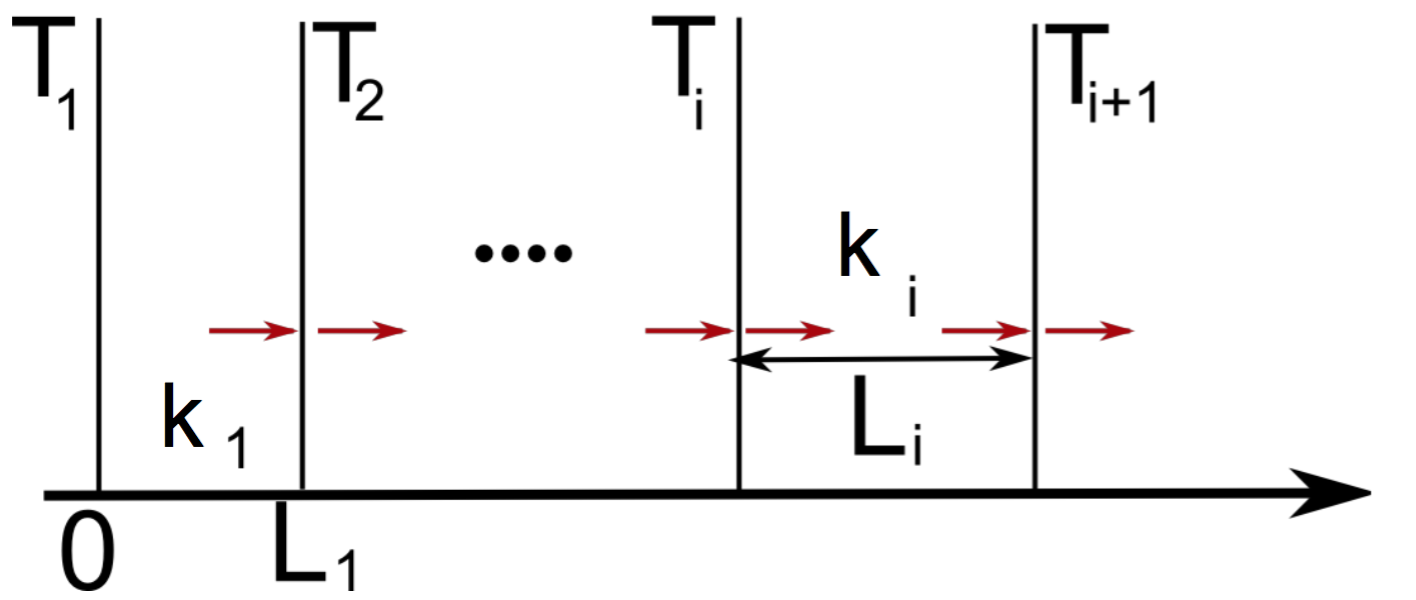
\includegraphics[scale=0.2]{ch3/6}
 				\end{wrapfigure}
 				By assuming the temperature continuity and the flux conservation at the boundary of each wall, we have 
 				\begin{equation}
 					\dot{Q} = \frac{T_1-T_{n+1}}{R} \qquad with \qquad R =\sum R_i = \sum \frac{L_i}{k_iA}
 				\end{equation}
 				
 			\subsection{Adding two extra resistance - the Biot number}
 				\label{sec:3.3.3}
 				\begin{wrapfigure}[5]{l}{5.8cm}
 				\vspace{-5mm}
 				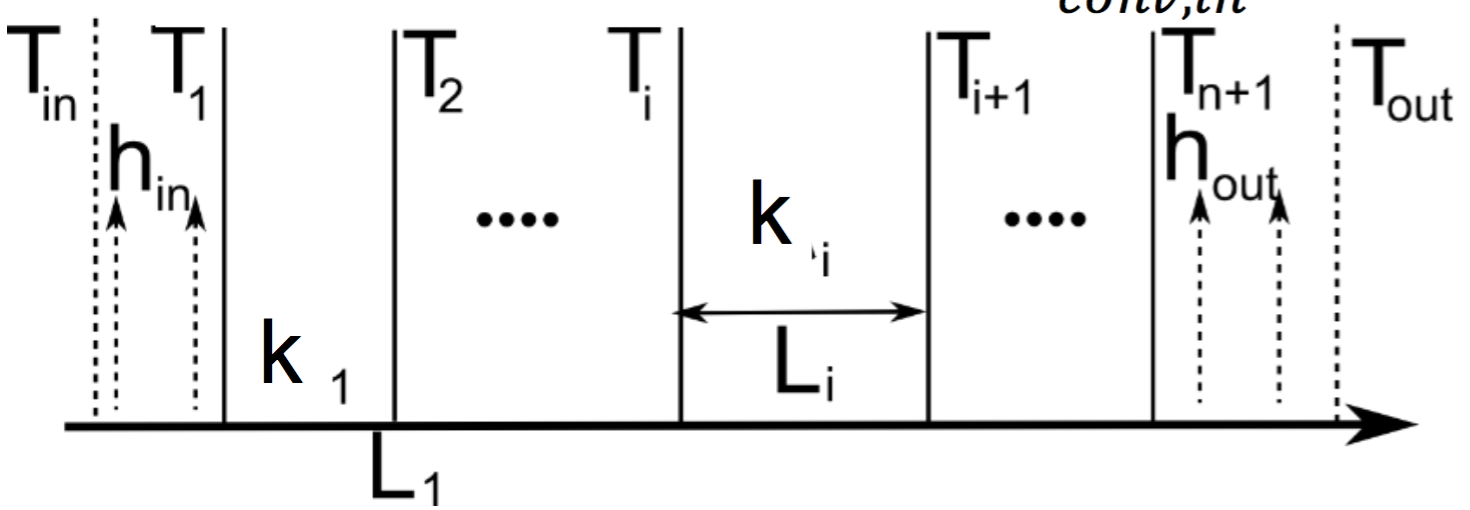
\includegraphics[scale=0.22]{ch3/7}
 				\end{wrapfigure}
 				Close to the walls the convective effect appears and is described by 
 				\begin{equation}
 					\dot{q} = h_{in} (T_{in}-T_1) \quad and \quad \dot{q} = h_{out} (T_{n+1} - T_{out})
 				\end{equation}
 				and the heat transfer rate can be found like 
 				\begin{equation}
 					\dot{Q} = \frac{T_{in}-T_{out}}{R} \qquad and \qquad R = \frac{1}{h_{in}A} + \sum \frac{L_i}{k_iA} + \frac{1}{h_{out}}
 				\end{equation}
 				But is it important to take care of the convective effect ? Let's compare the convective and conductive effect in the inner side 
 				\begin{equation}
 					\left. 
 					\begin{aligned}
 					 	T_{in}-T_1 &= \frac{\dot{Q}}{h_{in} A} \\
 					 	T_1 - T_2 &= \frac{L_1\dot{Q}}{k_1A}
 					\end{aligned}
 					\right\} \Rightarrow \frac{T_1-T_2}{T_{in}-T_1} = \frac{L_1h_{in}}{k_1} = Bi
 				\end{equation}
 				That is the \textbf{Biot number} that compares the convection in the fluid around the solid to the conduction in the solid.
 			
 			\subsubsection{Bi << 1}
	 			\begin{wrapfigure}[2]{r}{3cm}
 				\vspace{-5mm}
 				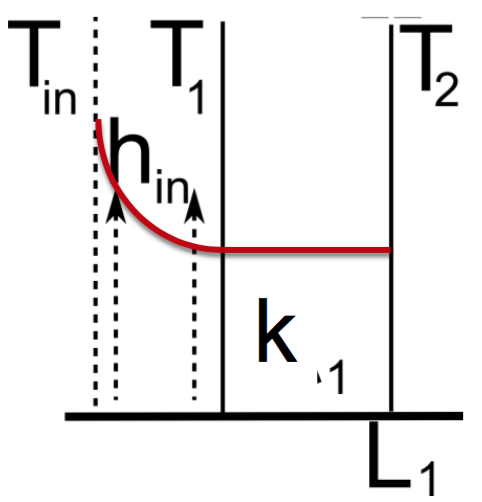
\includegraphics[scale=0.35]{ch3/8}
 				\end{wrapfigure}
 			It means that $k \gg h_{in}$ so that the convection is limiting and that the temperature difference is in the fluid. The variation of $T$ in the solid is negligible.\\\\
 			
 			 \subsubsection{Bi >> 1}
	 			\begin{wrapfigure}[3]{l}{3cm}
 				\vspace{-5mm}
 				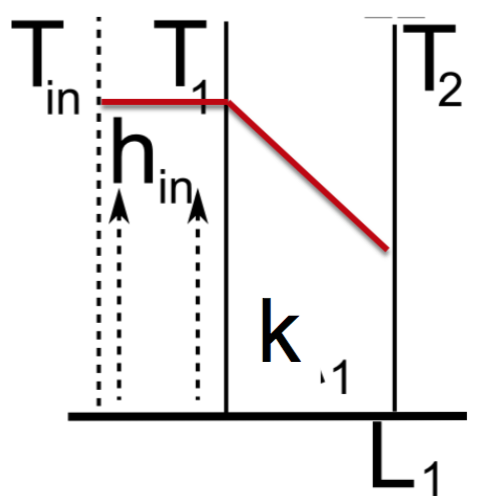
\includegraphics[scale=0.35]{ch3/9}
 				\end{wrapfigure}
 				In that case, the convection is dominating because $h_{in} \gg k$. The temperature difference is in the solid while the variation is in negligible in the fluid. \\\\\\
 			
	\subsection{Heat conduction in tubes}
	It's the same principle but in cylindrical coordinates. $\dot{Q}$ is conserved for all radius and is expressed like 
	\begin{equation}
		\dot{Q} = \dot{q}2\pi r H
		\label{eq:3.18}
	\end{equation}
 	The flow then writes 
 	\begin{equation}
 			\dot{Q} = \frac{T_1-T_2}{R}\qquad R = \frac{1}{2\pi r_1 H h_{in}} + \sum \frac{\ln (r_{i+1}/r_i)}{k_i 2\pi H} + \frac{1}{2 \pi r_{n+1}Hh_{out}}
 	\end{equation}
 	
\section{1D cylindrical problem with source term}
	\begin{wrapfigure}[8]{r}{2.5cm}
 	\vspace{-5mm}
 	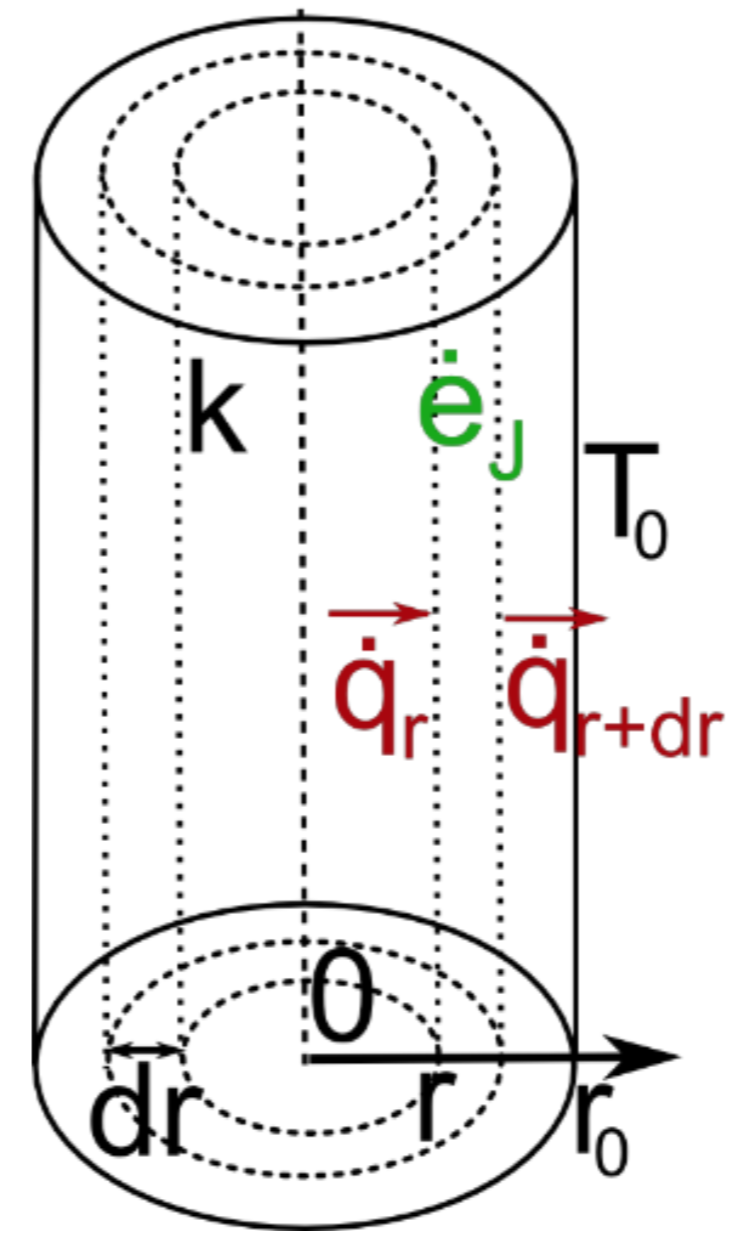
\includegraphics[scale=0.2]{ch3/11}
 	\end{wrapfigure}
	Let's consider an infinite cylindrical electric wire\footnote{Fil} of radius $r_0$ in an environment of temperature $T_0$. An electric current generates heat \textbf{uniformly} due to \textbf{Joule effect} at a volumetric rate $\dot{e}_J$ $[W/m^3]$. Let's do the heat balance along the radius
	\begin{equation}
		\cancel{Accumulation} = (In - Out) Fluxes + (Sources - \cancel{Sink})
	\end{equation}
	There are no accumulation because the system is stationary and nothing consume heat. Replacing by mathematical expression
	\begin{equation}
		\dot{Q}_r = \dot{Q}_{r+dr} - \dot{e}_J 2\pi r H dr
	\end{equation}
	applying the first order Taylor expansion
	\begin{equation}
		\dot{Q}_{r+dr} = \dot{Q}_r + \frac{d\dot{Q}_r}{dr}dr \qquad \Rightarrow \qquad \frac{d\dot{Q}_r}{dr} = \dot{e}_J 2\pi rH 
	\end{equation}
	Combining with the Fourier law and equation \autoref{eq:3.18} 
	\begin{equation}
		\frac{d}{dr}\left(-k 2\pi rH\frac{dT}{dr}\right) = \dot{e}_J 2\pi r H \qquad \Leftrightarrow \qquad \frac{k}{r}\frac{d}{dr}\left(r\frac{dT}{dr}\right) = -\dot{e}_J
	\end{equation}
	The integration gives the result 
	\begin{equation}
		T = \frac{-\dot{e}_J}{4k}r^2 + C_1 \ln (r) +C_2
	\end{equation}
	and after applying the boundary conditions $r = 0 \rightarrow T \ finite$ and $r = r_0 \rightarrow T = T_0$
	\begin{equation}
		T = T_0 + \frac{\dot{e}_Jr_0^2}{4k}\left( 1-\frac{r^2}{r_0^2} \right)
	\end{equation}
	
	\begin{wrapfigure}[5]{l}{4cm}
	\vspace{-10mm}
	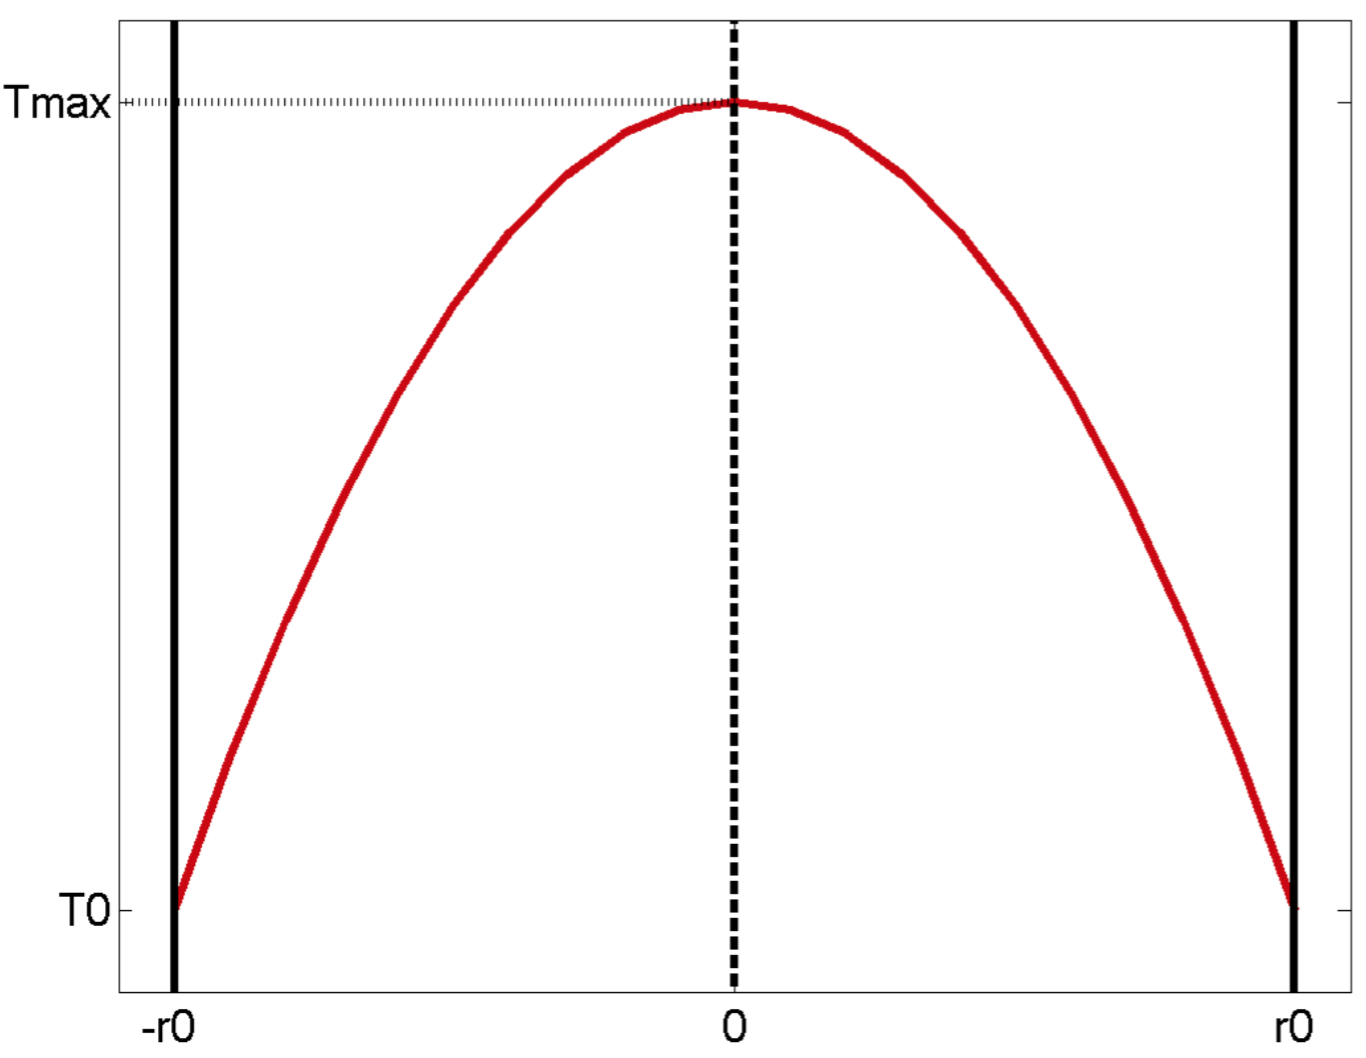
\includegraphics[scale=0.15]{ch3/12}
	\end{wrapfigure}
	$T_{max} = T_0 + \frac{\dot{e}_Jr_0^2}{4k}$ is obtained in the middle of the cylinder, so there is a moving heat. It's logical to have an equation depending on $r_0$ because if the radius increases, it will be more difficult for heat to reach the external environment. \\
	
\section{Generalization : unstationary 3D heat balance with heat generation - The second Fourier law}
	\begin{wrapfigure}[9]{r}{4cm}
	\vspace{-10mm}
	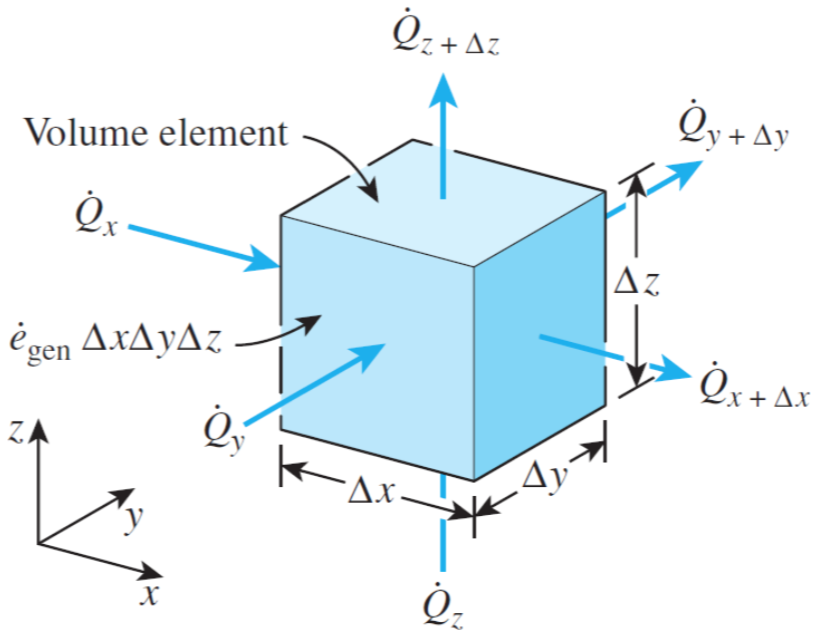
\includegraphics[scale=0.4]{ch3/13}
	\end{wrapfigure}	
	Always the same principle
	\begin{equation}
		Accumulation = (In - Out) Fluxes + (Sources - Sink)
	\end{equation}		
	replaced by mathematical expressions
	\begin{equation}
		\rho c_p\frac{\partial T}{\partial t} + \frac{\partial}{\partial x} \left( k \frac{\partial T}{\partial x} \right) + \frac{\partial}{\partial y} \left( k \frac{\partial T}{\partial y} \right) + \frac{\partial}{\partial z} \left( k \frac{\partial T}{\partial z} \right) + \dot{e}_{gen} = 0
	\end{equation}
	Using the definition of thermal diffusivity $\alpha = \frac{k}{\rho c_p}$, we obtain the \textbf{second Fourier law}
	\begin{equation}
		\frac{\partial T}{\partial t} + \nabla (\alpha \nabla T) + \dot{e}_{gen} = 0 
	\end{equation}
	There is the 5 classical boundary conditions to use with the Fourier law : 
	\begin{enumerate}
		\item Fixed temperature : $T = T_0$
		\item Fixed flux density : $\dot{q} = -k \frac{dT}{dx} = \dot{q}_0$
		\item Continuity of the flux : $\dot{q}_1 = -k_1\frac{dT}{dx}|_1 = \dot{q}_2 = -k_2\frac{dT}{dx}|_2$
		\item Convection at the boundary : $\dot{q} = -k\frac{dT}{dx} = h(T-T_b)$
		\item If we look at an insulated material : $\frac{dT}{dx} = 0 $
	\end{enumerate}
	
	